
%\documentclass[mathserif]{beamer}
\documentclass[handout]{beamer}
%\usetheme{Goettingen}
%\usetheme{Warsaw}
\usetheme{Singapore}



%\usetheme{Frankfurt}
%\usetheme{Copenhagen}
%\usetheme{Szeged}
%\usetheme{Montpellier}
%\usetheme{CambridgeUS}
%\usecolortheme{}
%\setbeamercovered{transparent}
\usepackage[english, activeacute]{babel}
\usepackage[utf8]{inputenc}
\usepackage{amsmath, amssymb}
\usepackage{dsfont}
\usepackage{graphics}
\usepackage{cases}
\usepackage{graphicx}
\usepackage{pgf}
\usepackage{epsfig}
\usepackage{amssymb}
\usepackage{multirow}	
\usepackage{amstext}
\usepackage[ruled,vlined,lined]{algorithm2e}
\usepackage{amsmath}
\usepackage{epic}
\usepackage{epsfig}
\usepackage{fontenc}
\usepackage{framed,color}
\usepackage{palatino, url, multicol}
%\algsetup{indent=2em}
\newcommand{\factorial}{\ensuremath{\mbox{\sc Factorial}}}
\newcommand{\BIGOP}[1]{\mathop{\mathchoice%
{\raise-0.22em\hbox{\huge $#1$}}%
{\raise-0.05em\hbox{\Large $#1$}}{\hbox{\large $#1$}}{#1}}}
\newcommand{\bigtimes}{\BIGOP{\times}}
\vspace{-0.5cm}
\title{Natural Language Processing \\ Introduction}
\vspace{-0.5cm}
\author[Felipe Bravo Márquez]{\footnotesize
%\author{\footnotesize  
 \textcolor[rgb]{0.00,0.00,1.00}{Felipe Bravo-Marquez}} 
  
 

\date{\today}

\begin{document}
\begin{frame}
\titlepage


\end{frame}


\begin{frame}{Disclaimer}
\begin{scriptsize}
\begin{itemize}
 \item  A significant part of the content presented in these slides is taken from other resources such as textbooks and publications.  
 \item  The neural network part of the course is heavily based on this book:
   \begin{figure}[h]
        	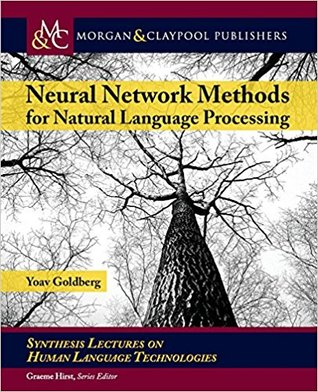
\includegraphics[scale = 0.4]{pics/goldbergNLP.jpg}
        \end{figure}
\end{itemize}
\end{scriptsize}

 
\end{frame}


\begin{frame}{Natural Language Processing}
\begin{scriptsize}
\begin{itemize}

\item The amount of digitalized textual data being generated every day is huge (e.g, the Web, social media, medicar records, digitalized books).

\item So does the need for translating, analyzing, and managing this flood of words and text.

\item Natural language processing (NLP) is the field of designing methods and algorithms that take as input or produce as output unstructured, \textbf{natural language data}. \cite{goldberg2017neural}

     \begin{figure}[h]
        	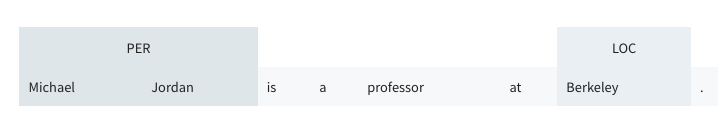
\includegraphics[scale = 0.4]{pics/NER.png}
        	\caption{Example: Named Entity Recognition}
        \end{figure}

\item Human language is highly ambiguous: \emph{I ate pizza with friends} vs. \emph{I ate pizza with olives}.

\item It is also ever changing and evolving (e.g, Hashtags in Twitter). 

\end{itemize}
\end{scriptsize}
\end{frame}


\begin{frame}{Natural Language Processing and Computational Linguistics}
\begin{scriptsize}
Natural language processing (NLP) develops methods for solving practical problems involving language \cite{JohnsonMLSS}.

\begin{itemize}
\item Automatic speech recognition.
\item Machine translation.
\item Information extraction from documents.
\end{itemize}

Computational linguistics (CL) studies the computational processes underlying (human) language.

\begin{itemize}
 \item How do we understand language?
 \item How do we produce language?
 \item How do we learn language?
\end{itemize}

Similiar methods and models are used in NLP and CL
\end{scriptsize}
\end{frame}



\begin{frame}{Linguistics levels of description}
\begin{scriptsize}
The field of \textbf{linguistics} includes subfields that concern themselves with different levels or aspects of the structure of \textbf{language}, as well as subfields dedicated to studying how linguistic structure interacts with human cognition and society \cite{bender2013linguistic}.
\begin{enumerate}
 \item \textbf{Phonetics}: The study of the sounds of human language.
 \item \textbf{Phonology}: The study of sound systems in human languages.
 \item \textbf{Morphology}: The study of the formation and internal structure of words.
 \item \textbf{Syntax}: The study of the formation and internal structure of sentences.
 \item \textbf{Semantics}: The study of the meaning of sentences
 \item \textbf{Pragmatics}: The study of the way sentences with their semantic meanings are
used for particular communicative goals.
\end{enumerate}


\end{scriptsize}
\end{frame}



\begin{frame}{Phonetics}
\scriptsize{
\begin{itemize}
 \item Phonetics studies the sounds of a language \cite{JohnsonMLSS}
 \item It deals with the organs of sound production (e.g., mouth, tongue, throat, nose, lips, palate)
\item Vowels vs consonants.
\item Vowels are produced with little restriction of the airflow from the lungs out
the mouth and/or the nose. \cite{fromkin2018introduction}
\item Consonants are produced with some restriction or closure in the vocal tract that
impedes the flow of air from the lungs. \cite{fromkin2018introduction}
\item International Phonetic Alphabet (IPA):  alphabetic system of phonetic notation. 
\end{itemize}
}
\end{frame}


\begin{frame}{Phonology}
\scriptsize{
\begin{itemize}
\item Phonology: The study of how speech sounds form patterns \cite{fromkin2018introduction}.
\item Phonemes are  the basic form of a sound (e.g., the phoneme /p/)
\item Example: Why \textbf{g} is silent in sign but is pronounced in the related word signature?
\item Example: English speakers pronounce /t/ differently (e.g., in water)
 
\end{itemize}
}
\end{frame}




\begin{frame}{Morphology}
\scriptsize{


\begin{itemize}
\item Morphology studies the structure of words (e.g.,re+structur+ing, un+remark+able) \cite{JohnsonMLSS}  
\item Morpheme: The linguistic term for the most elemental unit of grammatical form \cite{fromkin2018introduction}. Example morphology= morph + ology (the science of).
\item Derivational morphology: process of forming a new word from an existing word, often by adding a prefix or suffix 
\item Derivational morphology exhibits a hierarchical structure. Example: re+vital+ize+ation
     \begin{figure}[h]
        	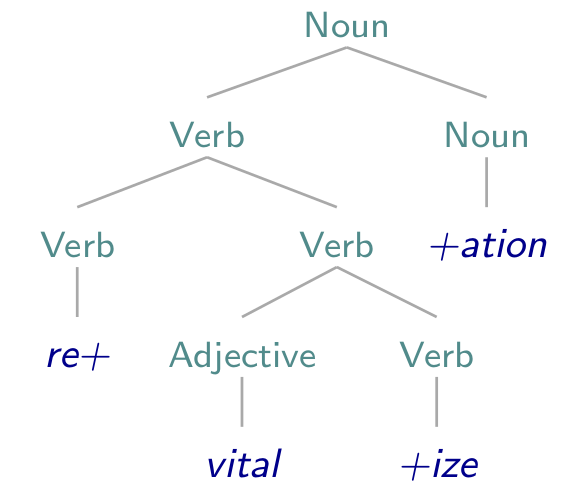
\includegraphics[scale = 0.2]{pics/morphology.png}
        \end{figure}
\item The suffix usually determines the syntactic category (part-of-speech) of the derived word.        
\end{itemize}

}


\end{frame}



\begin{frame}{Syntax}
\scriptsize{
\begin{itemize}
\item Syntax studies the ways words combine to form phrases and sentences \cite{JohnsonMLSS}
     \begin{figure}[h]
        	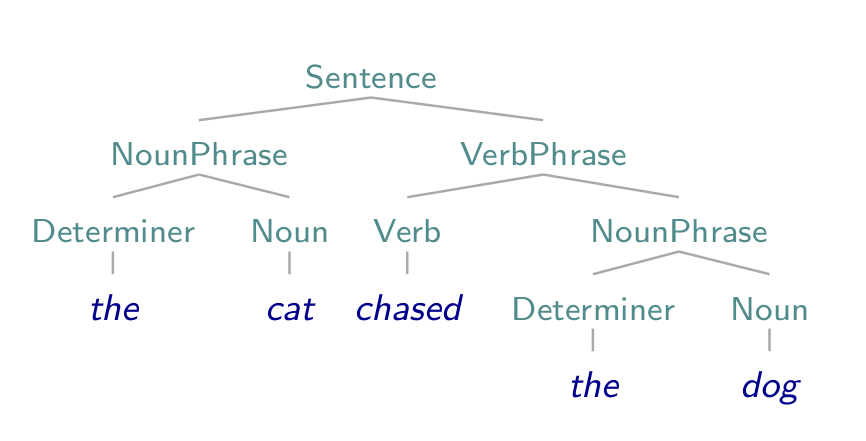
\includegraphics[scale = 0.3]{pics/parseTree1.png}
        \end{figure}
\item Syntactic parsing helps identify \textbf{who did what to whom}, a key step in
understanding a sentence.       
\end{itemize}

}


\end{frame}


\begin{frame}{Semantics}
\scriptsize{
\begin{itemize}
\item Semantics studies the meaning of words, phrases and sentences \cite{JohnsonMLSS}.
\item Semantic roles: indicate the role played by each entity in a sentence.
\item Examples of semantic roles: \textcolor[rgb]{0.00,0.00,1.00}{\textbf{agent}} (the entity that performs the action), \textcolor[rgb]{1.00,0.00,0.00}{\textbf{theme}} (the entity involved in the action), or \textcolor[rgb]{0.00,1.00,0.00}{\textbf{instrument}} (another entity used by the agent in order to perform the action).  
\item Annotated sentence: \textcolor[rgb]{0.00,0.00,1.00}{\textbf{The boy}}  cut \textcolor[rgb]{1.00,0.00,0.00}{\textbf{the rope}} with \textcolor[rgb]{0.00,1.00,0.00}{\textbf{a razor}}.
\item Lexical relations: relationship between different words \cite{yule2016study}.
\item Examples of lexical relations: synonymy (conceal/hide), antonymy (shallow/deep) and hyponymy (dog/animal).
\end{itemize}

}


\end{frame}



\begin{frame}{Pragmatics}
\scriptsize{
\begin{itemize}
\item \textbf{Pragmatics}: the study of how context affects meaning in certain situations \cite{fromkin2018introduction}.
\item Example: how the sentence ``It’s cold in here'' comes to be interpreted as ``close the windows''.
\item Example 2: Can you pass the salt?
\end{itemize}

}


\end{frame}


\begin{frame}{Natural Language Processing}
\begin{scriptsize}
\begin{itemize}

\item While we humans are great users of language, we are also very poor at formally understanding and describing the rules that govern  language.

\item  Understanding and producing language using computers is highly challenging.
\item The best known set of methods for dealing with language data rely on supervised machine learning.
\item Supervised machine learning: attempt to infer usage patterns and regularities from a set of pre-annotated input and output pairs (a.k.a training dataset).

\end{itemize}
\end{scriptsize}
\end{frame}


\begin{frame}[fragile]{Training Dataset: CoNLL-2003 NER Data}
Each line contains a token, a part-of-speech tag, a syntactic chunk tag, and a named-entity tag.
\begin{center}
\begin{semiverbatim}
U.N.         NNP  I-NP  I-ORG 
official     NN   I-NP  O
Ekeus        NNP  I-NP  I-PER
heads        VBZ  I-VP  O
for          IN   I-PP  O
Baghdad      NNP  I-NP  I-LOC
.            .    O     O
\end{semiverbatim}
\end{center}

\footnotemark{Source: \url{https://www.clips.uantwerpen.be/conll2003/ner/}}  

\end{frame}


\begin{frame}{Challenges of Language}
\begin{scriptsize}
\begin{itemize}
\item Three challenging properties of language: discreteness , compositionality, and sparseness.
\item \textbf{Discreteness}: we cannot infer the relation between two words from the letters they are made of (e.g., hamburger and pizza). 
\item \textbf{Compositionality}: the meaning of a sentence goes beyond the individual meaning of their words. 
\item \textbf{Sparseness}: The way in which words
(discrete symbols) can be combined to form meanings is practically infinite.
\end{itemize}
\end{scriptsize}
\end{frame}










\begin{frame}{Example of NLP Task: Topic Classification}
\begin{scriptsize}
\begin{itemize}
\item Classify a document into one of four categories: Sports, Politics, Gossip, and Economy. 
\item The words in the documents provide very strong hints.
\item Which words provide what hints? 
\item Writing up rules for this task is rather challenging. 
\item However, readers can easily categorize a number of documents into its topic (data annotation).
\item A supervised machine learning algorithm come up with the patterns of word usage that help categorize the documents.
\end{itemize}
\end{scriptsize}
\end{frame}


\begin{frame}{Example 3: Sentiment Analysis}
\begin{scriptsize}\begin{itemize}
 \item Application of \textbf{NLP} techniques to identify and extract subjective information from textual datasets.
\end{itemize}

\begin{block}{Main Problem: Message-level Polarity Classification (MPC)}
  \begin{enumerate}
   \item Automatically classify a sentence to classes \textcolor[rgb]{0.00,0.00,1.00}{\textbf{positive}}, \textcolor[rgb]{1.00,0.00,0.00}{\textbf{negative}}, or \textcolor[rgb]{0.00,1.00,0.00}{\textbf{neutral}}. 
   
     \begin{figure}[h]
        	
\includegraphics[scale = 0.15]{pics/sent.png}
        \end{figure}
   
   \item State-of-the-art solutions use \textbf{supervised} machine learning models trained from \textbf{manually} annotated examples \cite{Mohammad2013}.
  \end{enumerate} 
\end{block}

\end{scriptsize}

\end{frame}


\begin{frame}{Sentiment Classification via Supervised Learning and BoWs Vectors}

\begin{figure}[h]
        	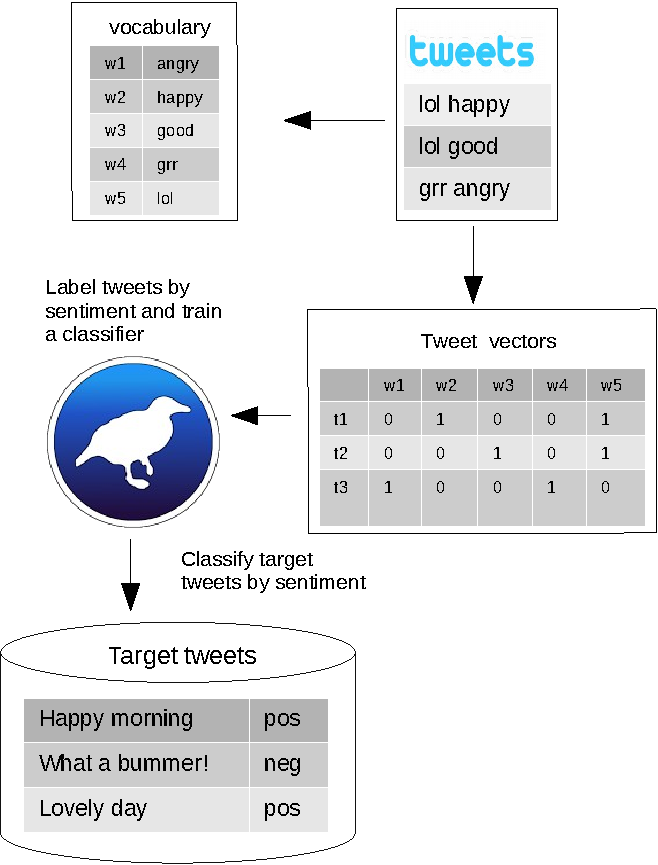
\includegraphics[scale = 0.5]{pics/bagOfwordsClassification.pdf}
        \end{figure}

\end{frame}




\begin{frame}{Supervised Learning: Support Vector Machines (SVMs)}
\begin{scriptsize}

\begin{itemize}


\item Idea: Find a hyperplane that separates the classes with the maximum margin (largest separation). 

     \begin{figure}[h]
        	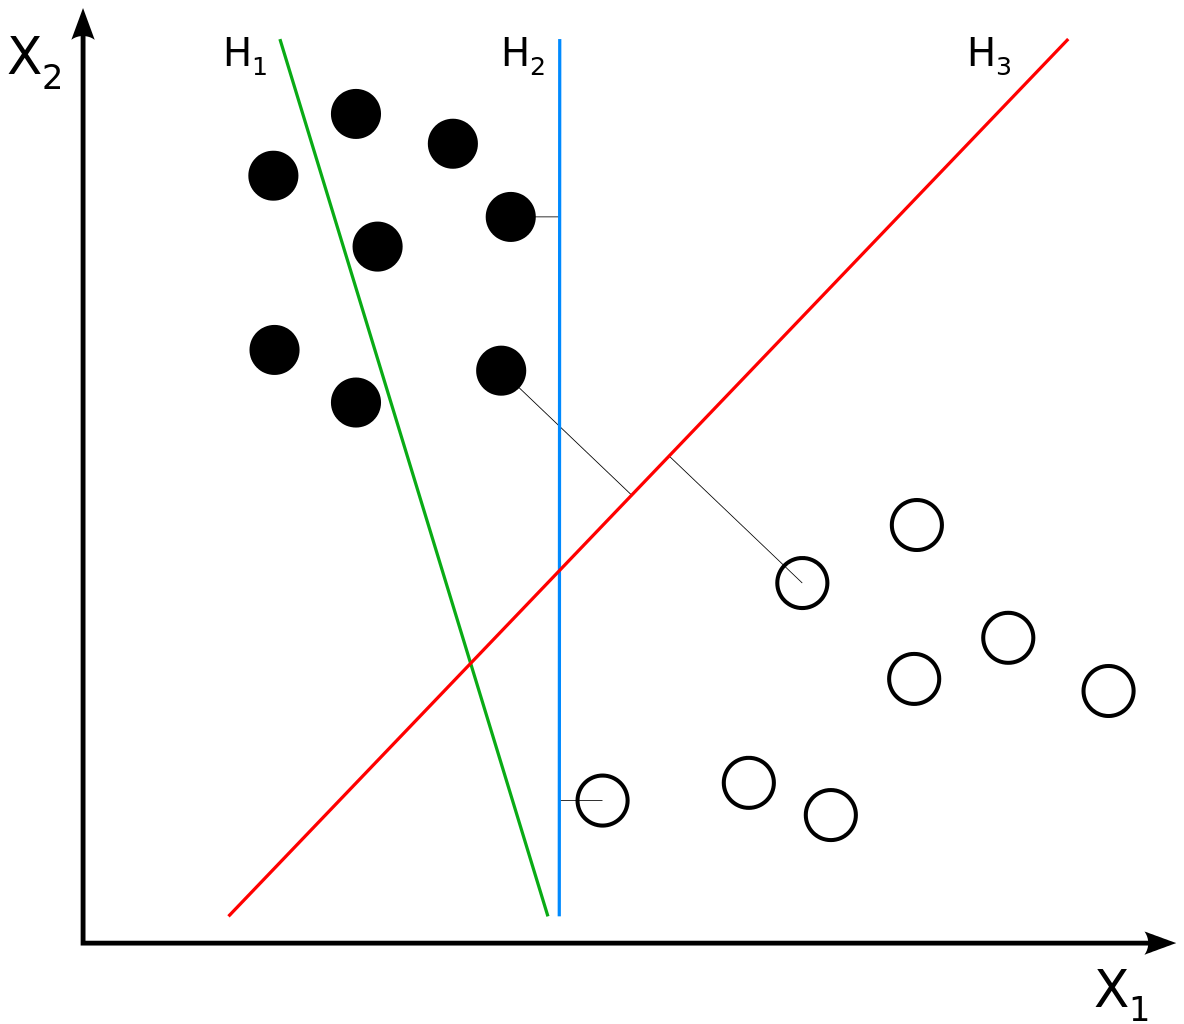
\includegraphics[scale = 0.15]{pics/SVM.png}
        \end{figure}

\item   
$H_3$ separates the classes with the maximum margin. 

\end{itemize}

\footnotemark{Image source: Wikipedia}       
   
\end{scriptsize}

\end{frame}

\begin{frame}{Linguistics and NLP}
\begin{scriptsize}
  \begin{itemize}
   \item Knowing about linguistic structure is important for feature design
and error analysis in NLP \cite{bender2013linguistic}.

\item Machine learning approaches to NLP require features which can describe and generalize across particular instances of language use.
\item Goal: guide the machine learning algorithm to find correlations between language use and its target set of labels.
\item Knowledge about linguistic structures can inform the design of
features for machine learning approaches to NLP.
  \end{itemize}
\end{scriptsize}

 
\end{frame}




\begin{frame}{Challenges in NLP}
\begin{scriptsize}
  \begin{itemize}
   \item \textbf{Annotation Costs}: manual annotation is \textbf{labour-intensive} and \textbf{time-consuming}. 
   \item \textbf{Domain Variations}: the pattern we want to learn can vary from one corpus to another (e.g., sports, politics).
 
 \item A model trained from data annotated for one domain will \textbf{not necessarily} work on another one! 
\item Trained models can become outdated over time (e.g., new hashtags).
  \end{itemize} 



\begin{block}{Domain Variation in Sentiment}
\begin{enumerate}
\item  For me the queue was pretty \textcolor[rgb]{0.00,0.00,1.00}{\textbf{small}} and it was only a 20 minute wait I think but was so worth it!!! :D @raynwise
\item Odd spatiality in Stuttgart. Hotel room is so  \textcolor[rgb]{1.00,0.00,0.00}{\textbf{small}} I can barely turn around but surroundings are inhumanly vast \& long under construction.
\end{enumerate}
\end{block}


\end{scriptsize}

\end{frame}



\begin{frame}{Overcoming the data annotation costs}
\begin{scriptsize}
\begin{block}{Distant Supervision}
  \begin{itemize}
   \item Automatically \textbf{label} unlabeled data (\textbf{Twitter API}) using a heuristic method.
   \item \textbf{Emoticon-Annotation Approach (EAA)}: tweets with positive \textcolor[rgb]{0.00,0.00,1.00}{\textbf{:)}} or negative \textcolor[rgb]{1.00,0.00,0.00}{\textbf{:(}} emoticons are labelled according to the polarity indicated by the emoticon~\cite{Read2005}.
  \item The emoticon is \textbf{removed} from the content.
  \item The same approach has been extended using hashtags \#anger, and emojis.
\item Is not trivial to find distant supervision techniques for all kind of NLP problems.
\end{itemize} 
 
\end{block}

\begin{block}{Crowdsourcing}
  \begin{itemize}
\item Rely on services like \textbf{Amazon Mechanical Turk} or \textbf{Crowdflower} to ask the \textbf{crowds} to annotate data.
\item This can be expensive.
\item It is hard to guarantee quality. 
   \end{itemize} 
 
\end{block}

\end{scriptsize}

\end{frame}




\begin{frame}{Sentiment Classification of Tweets}
\begin{scriptsize}
\begin{itemize}
\item In 2013, The Semantic Evaluation (SemEval) workshop organised the
``Sentiment Analysis in Twitter
task'' \cite{Semeval2013}.
 \item The task was divided into two sub-tasks: the expression
level and the message level. 
\item Expression-level: focused on determining
the sentiment polarity of a message according to a marked entity within
its content.
\item Message-level: the polarity has to be determined according to
the overall message.
\item  The organisers released training and testing datasets
for both tasks.
\cite{Semeval2013}
\end{itemize}
\end{scriptsize}
\end{frame}

%Tradi7onal: Curated sentiment dictionaries combined with either bag-of-words representa7ons (ignoring word order) or hand-designed nega7on features (aint gonna capture everything) 

% http://cs224d.stanford.edu/lectures/CS224d-Lecture1.pdf

\begin{frame}{The NRC System}
\begin{scriptsize}
\begin{itemize}
\item The team that achieved the highest performance in both
tasks among 44 teams was the \emph{NRC-Canada} team
\cite{Mohammad2013}.  
\item The team proposed a supervised approach using a linear SVM
classifier with the following hand-crafted features for representing tweets:
\begin{enumerate}
\begin{scriptsize}
\item  Word $n$-grams.
\item  Character $n$-grams. 
\item Part-of-speech tags.
\item Word clusters trained with the Brown clustering method~\cite{brown1992class}.
\item The number of elongated words (words with one character repeated more than two times).
\item The number of words with all characters in uppercase.
\item The presence of positive or negative emoticons.
\item The number of individual negations.
\item The number of contiguous sequences of dots, question marks and exclamation marks.
\item Features derived from polarity lexicons~\cite{Mohammad2013}. Two of these lexicons were generated using the PMI method from tweets annotated with hashtags and emoticons.
\end{scriptsize} 
\end{enumerate}
\end{itemize}
\end{scriptsize} 
\end{frame}




\begin{frame}{Feature Engineering and Deep Learning}
\begin{scriptsize}
\begin{itemize}
\item Designing the features of a winning NLP system requires a lot of domain-specific knowledge.
\item The NRC system was built before deep learning became popular in NLP.
\item Deep Learning systems on the other hand rely on representation learning to automatically learn good representations.
\item Large amounts of training data and faster multicore CPU/GPU machines are key in the success of deep learning. 
\item \textbf{Neural networks} and \textbf{word embeddings} play a key role in modern  architectures for NLP.

\end{itemize}
\end{scriptsize}
\end{frame}


\begin{frame}{Deep Learning and Linguistic Concepts}
\begin{scriptsize}
\begin{itemize}
\item If deep learning models can learn representations automatically, are linguistic concepts still useful (e.g., syntax, morphology)?
\item Some proponents of deep-learning argue that such inferred, manually designed, linguistic properties are not needed, and that the neural network will learn
these intermediate representations (or equivalent, or better ones) on its own \cite{goldberg2016primer}. 
\item The jury is still out on this.
\item Goldberg believes many of these linguistic concepts can indeed be inferred by the network on its own if given enough data.
\item However, for many other cases we do not have enough training data available for the task we care about, and in these cases providing the network with the more explicit general concepts can be very valuable.
\end{itemize}
\end{scriptsize}
\end{frame}


\begin{frame}{History}
\begin{scriptsize}
\begin{itemize}
\item NLP progress can be divided into three main waves: 1) rationalism, 2) empiricism, and 3) deep learning \cite{deng2018deep}.
\end{itemize}
\end{scriptsize}
\end{frame}



\begin{frame}{Roadmap}
In this course we will introduce modern concepts in natural language processing based on \textbf{statistical models} (second wave) and \textbf{neural networks} (third wave). The main concepts to be convered are listed below:
\begin{scriptsize}
\begin{enumerate}
\item Text classification.
\item Linear Models.
\item Naive Bayes.
\item Hidden Markov Models.
\item Neural Networks.
\item Word embeddings.
\item Convolutional Neural Networks (CNNs) 
\item Recurrent Neural Networks: Elman, LSTMs, GRUs. 
\item Attention.
\item Sequence-to-Sequence Models.
\item Parse Trees.
\end{enumerate} 
\end{scriptsize}
\end{frame}



\begin{frame}{Important Websites}

\begin{scriptsize}
\begin{enumerate}
\item \url{http://nlpprogress.com/}
\item \url{https://allennlp.org/}
\end{enumerate} 
\end{scriptsize}
\end{frame}




\begin{frame}
\frametitle{Questions?}
%\vspace{1.5cm}
\begin{center}\LARGE Thanks for your Attention!\\ \end{center}



\end{frame}

\begin{frame}[allowframebreaks]\scriptsize
\frametitle{References}
\bibliography{bio}
\bibliographystyle{apalike}
%\bibliographystyle{flexbib}
\end{frame}  


%%%%%%%%%%%%%%%%%%%%%%%%%%%

\end{document}
